\documentclass[../dissertation.tex]{subfiles}

\begin{document}

\chapter{The Expected Sarsa and Neural-Q Path Tracers}
\label{chap:td_deep_sampling}

Monte Carlo Integration, importance sampling, path tracing, and reinforcement learning have all been introduced. So now it is finally time to combine all of these concepts to build path tracing algorithms which importance sample directions to continue light paths in to reduce image noise.

In this section we introduce two modified path tracers. The first is based on the NVIDIA path tracer, which we refer to as the Expected Sarsa path tracer. The other is our newly proposed path tracer which we refer to as the Neural-Q path tracer. Both path tracers progressively learn the incident radiance function for importance sampling directions to continue light paths in. This reduces the variance in the Monte Carlo approximation of a pixels colour, ultimately reducing the noise in rendered images. However, the Expected Sarsa path tracer learns the incident radiance function for a discrete set of locations in the scene, whereas our Neural-Q path tracer learns it for the continuous set of locations in a scene.

\section{The Expected Sarsa Path Tracer}
\label{sec:expecte_sarsa_path_tracer}

In this section we introduce the Expected Sarsa path tracer proposed by NVIDIA in \cite{dahm2017learning}. In doing so, we will cover how light transport can be linked to the rendering equation for learning the incident radiance function, the Irradiance Volume data structure, and the modified path tracing algorithm itself.

\subsection{Linking TD-Learning and Light Transport Simulation}
\label{sec:td_light_transport}
Here, we will  link together the concepts introduced in chapter \ref{chap:technical} to derive a way of learning the incident radiance on any position in the scene $x$ from any direction $\omega$. In other words, we will step through the derivation of the learning rule given in \cite{dahm2017learning} for learning the incident radiance function based on the TD-learning method Expected Sarsa.

First, the Expected Sarsa learning rule's summation over the set of all actions $\mathcal{A}$ can be represented as an integral with respect to an action $a$ over all actions $\mathcal{A}$, as shown in Equation \ref{eq:sarsa_integral}.

\begin{align}
Q(S_t, A_t) & \leftarrow Q(S_t, A_t) + \alpha [R_{t+1} + \gamma \sum_a \pi(a| S_{t+1}) Q(S_{t+1}, a) - Q(S_t, A_t)]\\
& =  (1 - \alpha) \cdot Q(S_{t},A_t) + \alpha \cdot \left( R_{t+1} + \gamma \sum_a \pi(a|S_{t+1}) Q(S_{t+1}, a) \right)\\
& = (1 - \alpha) \cdot Q(S_{t},A_t) + \alpha \cdot \left( R_{t+1} + \gamma \int_\mathcal{A} \pi(a|S_{t+1}) Q(S_{t+1}, a) da \right)
 \label{eq:sarsa_integral}
\end{align}

\noindent
Recall the rendering equation from section \ref{sec:rendering_equation} describes the radiance in an outgoing direction $\omega$ from point $x$ is equivalent to the emitted radiance in $\omega$ from $x$ plus the reflected radiance in the $\omega$ from $x$. Note, we have set the incident radiance function to $L_i(x, \omega_i) = L_o(h(x, \omega_i), -\omega_i)$ (see section \ref{sec:rendering_equation}).

\begin{equation}
L_o(x, \omega) = L_e(x,\omega)  + \int_\Omega L_o(h(x, \omega_i), -\omega_i)  \cdot f_r(\omega_i, x, \omega) \cdot \cos(\theta_i) d\omega_i \nonumber
\end{equation}

\noindent
Now, by matching  terms from the rendering equation to the Expected Sarsa learning rule in equation \ref{eq:sarsa_integral}, equation \ref{eq:expected_sarsa_td_learning} is formed. Where this new learning rule is designed to approximate the incident radiance in direction $\omega$ on a point $x$ in the scene. Therefore, the Q-value of the state-action pair $Q(x = S_t, \omega = A_t)$ is determined by the amount of radiance incident in direction $\omega$ on $x$. An important detail which may be overlooked is that the substitution of $\gamma \cdot \pi(a|S_{t+1})$ for $f_s(\omega_k, y, -\omega) \cdot \cos(\theta_i)$ ensures that a trade off of long term rewards for more immediate rewards is made as $f_s(\omega_k, y, -\omega) \cdot \cos(\theta_i) \leq 1$. Meaning, the learning rule accurately accounts for a light paths loss of energy as reflects off surfaces within the scene.

Below, we have listed what each term in the Expected Sarsa learning rule is matched to for deriving equation \ref{sec:expected_sarsa_td_learning}:
\begin{conditions}
 S_t &  3D position in the scene, $x \in \mathbb{R}^3$  \\
 
 A_t & Sampling a direction to continue the light path in from location $x$, in direction $\omega$ \\   
 
S_{t+1}   &  3D position of a light ray from reflected from $x$ in direction $\omega$, $y = h(x, \omega)$ \\

R_{t+1} & Emitted radiance from point $y$ in direction $-\omega$, $L_e(y, -\omega)$\\

\mathcal{A} & All directions in the hemisphere at $x$, oriented to the surface normal at $x$, $\Omega$\\

\gamma \cdot \pi(a|S_{t+1}) & BRDF and the cosine of the angle between $y$ and $\omega_i$, $f_r(\omega_i, y, \omega) \cdot \cos(\theta_i)$\\
    
Q(S_t, A_t) & Approximated radiance incident on $x$ from direction $\omega$, $-L_i(x, \omega) = Q(x, \omega)$\\
\end{conditions}

\begin{equation}
Q(x, \omega) \leftarrow (1 - \alpha) \cdot Q(x, \omega) + \alpha \cdot \left( L_e(y, -\omega) + \int_\Omega Q(y, \omega_i) f_s(\omega_i, y, -\omega) \cos(\theta_i) d\omega_i \right)
\label{eq:expected_sarsa_td_learning}
\end{equation}

Finally, Monte Carlo integration with a uniform distribution PDF can be used to approximate the integral in equation \ref{eq:expected_sarsa_td_learning}. This converts the action space from continuous to $m$ discrete angles and provides a numerical solution for approximating the incident radiance on $x$ from direction $\omega$, as shown in equation \ref{eq:mc_expected_sarsa_td_learning}.

\begin{equation}
Q(x, \omega) \leftarrow (1 - \alpha) \cdot Q(x, \omega) + \alpha \cdot \left( L_e(y, -\omega) +\frac{2 \pi}{m} \sum_{k=1}^{m-1} Q(y, \omega_k) f_s(\omega_k, y, -\omega) \cos(\theta_k)  \right)
\label{eq:mc_expected_sarsa_td_learning}
\end{equation}

The estimated incident radiance function for a point $x$ consists of $m$ approximated incident radaince values from directions $\omega_i \forall i = 1,...,m$. These approximated incident radiance values can be converted into a distribution. This distribution is an apporximation of the \textit{radiance distribution} for a point \cite{greger1998irradiance}. A good approximation of the radiance distribution at a point $x$ will have a similar shape to the true function of incident radiance at point $x$, $L_o(x, \omega)$ $\forall \omega \in \Omega$. Therefore, by MC importance sampling, sampling directions to continue light paths in from the learned radiance distribution and using it as the PDF in the MC approximation, will significantly reduce the variance in the approximation. Leading to a significant reduction in image noise. Figure \ref{fig:incident_radiance_distribution} gives an illustration of the radiance distribution for a point.

\begin{figure}[h]
\centering
\begin{minipage}{0.4\textwidth}
      \begin{tikzpicture}
	 \begin{axis}[every axis plot post/.append style={
	  mark=none,domain=-20:20,samples=200,smooth},
	  axis lines = left,
	  tick style={draw=none},
	  xticklabels={},
	  yticklabels={},
	    % All plots: from -2:2, 50 samples, smooth, no marks
	  axis x line*=bottom, % no box around the plot, only x and y axis
	  axis y line*=left, % the * suppresses the arrow tips
	  enlargelimits=upper,
	  xlabel = $\omega_i$,
	  ylabel = $p(\omega_i)$
	  ] % extend the axes a bit to the right and top
	  \addplot [
	  color=red,
	  ]{gauss(-10.0,4.0) + gauss(10.0,4.0)};
	\end{axis}
    \end{tikzpicture}
\end{minipage}
\caption{An illustration of a simple incident radiance distribution for a given point $x$ in a scene. Where $\omega_i$ $\forall \omega_i \in \Omega$ are all possible incident directions in the hemisphere around the point $x$ oriented to the surface normal at $x$.The scene contains two area lights with the same power which are visible from $x$ in the scene, causing two equal level peaks in the incident radiance distribution for $x$.}
  \label{fig:incident_radiance_distribution}
\end{figure}

\subsection{The Irradiance Volume}
The Expected Sarsa learning rule derived in equation \ref{eq:mc_expected_sarsa_td_learning} requires some sort of data-structure for looking up and updating the incident radiance on a point $x$ from direction $\omega_i$, which from here on we will refer to as a Q-value. Therefore, the main requirement of the data structure is that it has some way of representing a discrete set of angles ($\omega_k$ $\forall k = 1, ..., m$) in a hemisphere located at a position $x$ and oriented to the surface normal at $x$. The Irradiance Volume data structure \cite{greger1998irradiance} meets this requirement.\\

\begin{figure}[h]
\begin{center}
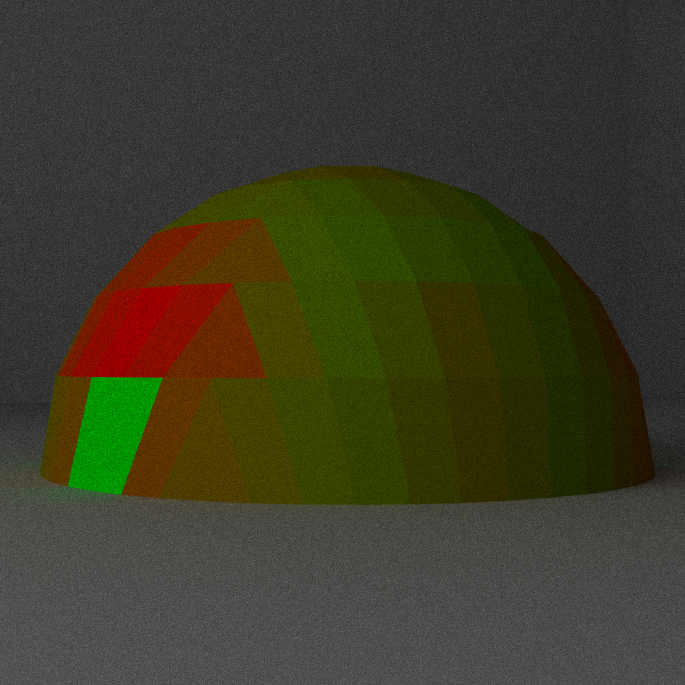
\includegraphics[width=0.3\textwidth]{images/renders/hemispheres/irradiance_volume.png}    
\end{center}
\caption{An Irradiance Volume. Each sector holds the incoming radiance $L_i(x,\omega_k)$, the more green a sector is the lower the stored radiance in that sector, the more red a sector is the higher the stored radiance in that sector. }
\label{fig:irradiance_volume}
\end{figure}

Originally designed to be used for pre-computation of radiance values which are looked up at runtime to approximate global illumination, the Irradiance Volume data structure is essentially a discretized version of a hemisphere which is visually represented in figure \ref{fig:irradiance_volume}. The image shows the discrete sectors which make up a hemisphere. This was implemented by converting a 2-dimensional square grid into the 3-dimensional hemisphere shown, which is known as an adaptive quadrature. Where all sectors in the 2-dimensional grid have an equal area and a mapping introduced in \cite{shirley1994notes} converts the 2-dimensional grid coordinates into a hemisphere made up of sectors in 3-dimensional space. The mapping ensures the hemisphere sectors remain equal to one another, meaning the discrete set of direction represented by the hemisphere are of equal angles apart from one another.

\begin{figure}[!htb]
\centering
\minipage{0.32\textwidth}
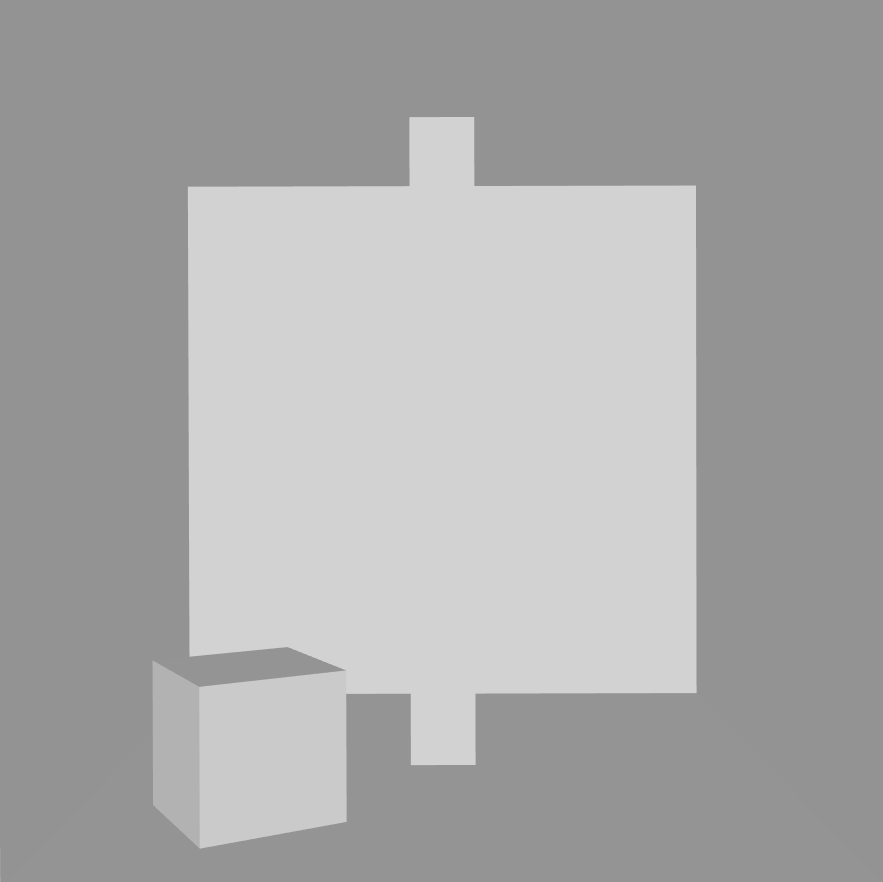
\includegraphics[width=1\textwidth]{images/renders/simple_room/geometry.png}
  \subcaption{Representation of the scenes geometry meshes}
\endminipage\hfill
\minipage{0.32\textwidth}
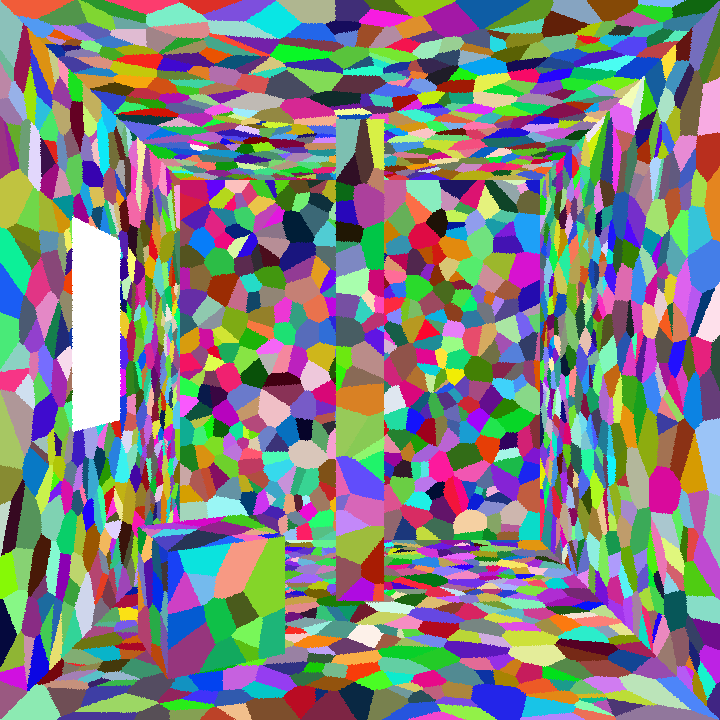
\includegraphics[width=1\textwidth]{images/renders/simple_room/voronoi.png}
   \subcaption{Voronoi Plot of Irradiance Volume locations}
\endminipage\hfill
\minipage{0.32\textwidth}
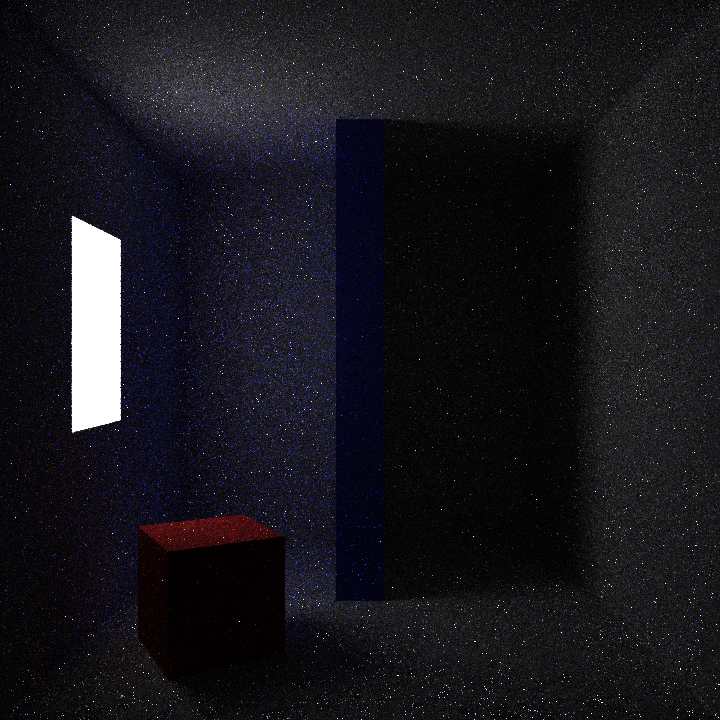
\includegraphics[width=1\textwidth]{images/renders/simple_room/reinforcement_16.png}
  \subcaption{Expected Sarsa path tracer with 16 SPP}
\endminipage
\caption{An example of discretizing location in the scene into Irradiance Volume locations. The geometry mesh (a) is used to uniformly sample Irradiance volume positions. Image (b) shows a voronoi plot for the Irradiance Volumes in the scene, where each pixel is coloured to the represent its closest Irradiance Volume, so each sector of colour in (b) represents a different Irradiance Volume location. Finally (c) gives a render using the Expected Sarsa path tracer based on Algorithm \ref{alg:expected_sarsa_pathtracer}.}
\label{fig:scene_discretization_example}
\end{figure}

Each sector of the Irradiance Volume is then used to store the current approximation of incident radiance in the direction formed by the unit vector travelling from centre of the sector to the centre of the hemisphere. Therefore, an Irradiance Volume stores the incident radiance (Q-value) for a given position $x$ (state) in the scene, from each direction $\omega_k$ (action), for all sectors $\forall k = 1,...,m$ in the hemisphere located at $x$. 

In order to store Q-values across the scene, Irradiance Volumes can be uniformly sampled over the scenes geometry as shown in figure \ref{fig:scene_discretization_example}. Then, to lookup a radiance/Q-value for a given position $x$ in direction $\omega_k$, a nearest neighbour search is performed to find the closest Irradiance Volume to position $x$,followed by a lookup to retrieve the Q-value from the sector at index $k$. Using this method results in a lookup and update time of $O(\log n) + O(1) = O(\log n)$ when using the KD-Tree data structure for nearest neighbour search \cite{bentley1975multidimensional}. A KD-Tree is essentially a binary tree for nearest neighbour search in $n$-dimensional space. 

Lookup and update procedures from the Irradiance volumes in the scene are all that are needed to apply the Expected Sarsa learning rule in equation \ref{eq:mc_expected_sarsa_td_learning}. The entire collection of Irradiance Volumes in a scene can be thought of as a large 5-dimensional table ($x \in \mathbb{R}^3, \omega \in \mathbb{R}^2$) to store the incident radiance approximations. This table is our Q-table (see section \ref{sec:td_learning}) which is used by the Expected Sarsa learning rule to approximate the incident radiance function.

Each radiance volume also stores the radiance distribution approximated for its centre point. This is calculated by normalizing its stored incident radiance values (Q-values) into a probability distribution. As described in section \ref{sec:td_light_transport}, a direction to continue a light path in can be sampled proportionally to the radiance distribution of the closest radiance volume to the a light paths intersection point. This distribution is also used as the PDF for calculating the MC approximation of a pixels colour value in path tracing (equation \ref{eq:rendering_eq_monte_carlo}).

To summarize all Irradiance Volumes combined (Q-table) store both the current approximation of the incident radiance function, as well as a PDF which is the approximated incident radiance function normalized. Meaning, if the approximation of the incident radiance function becomes more accurate, the stored PDF will come closer to normalizing the the true incident radiance function. This will lead to a reduction in variance of the MC approximation of pixel colour values, leading to a fall in image noise. Exactly how we go about updating the incident radiance distribution is what we will cover in section \ref{sec:expected_sarsa_path_tracer}.

\subsection{Expected Sarsa Path Tracing}
\label{sec:expected_sarsa_path_tracer}

The Expected Sarsa path tracing algorithm is very similar to the original forward path tracer introduced in algorithm \ref{alg:forward_path_tracing}. The algorithm learns online, meaning after every rendered frame, pixel values are likely to have a lower variance due to am improvement in the approximation of the learned incident radiance function $L_i$ stored in the Q-table formed by all Irradiance Volumes in the scene. Initially, Irradiance Volumes are sampled uniformly across the room with all Q-values initialised to a small constant proportional to the number of sectors on each hemisphere $m$. This encodes the assumption that initially the radiance incident in all directions at any given point in the scene is equal. This a reasonable assumption, as initially we have no prior knowledge of any radiance values $Q(x, \omega_k)$. With the radiance volumes set up, every frame $N$ light paths are sampled from the camera, through each pixel and into the scene. This process determines the pixels average colour estimate using algorithm \ref{alg:expected_sarsa_pathtracer}. Algorithm \ref{alg:expected_sarsa_pathtracer} updates the radiance distribution stored in each Irradiance Volume after every rendered frame using the updated $Q(x, \omega_k)$ values stored. Meaning the next frame will importance sample from the Irradiance Volumes updated radiance distributions. The three additions to algorithm  \ref{alg:forward_path_tracing} to form the Expected Sarsa path tracer are given below.

\subsubsection*{Addition 1: Sample directions proportional to closest radiance distribution}
The direction to continue the light path in is sampled proportional to the radiance distribution held in the nearest Irradiance Volume to the intersection location $y$. In practice, the stoed radiance distirbution at every Irradiance Volume is a set of discrete normalized Q-values corresponding to the discrete directions $\omega_k$ $\forall k = 1, ..., m$. Therefore inverse transform sampling \cite{devroye2006nonuniform} is used to sample a direction from the stored radiance distribution. Inverse transform sampling is where a random number $r \in [0,1]$ is sampled, then the largest number $x$ from the domain of the cumulative distribution $P(X)$ is returned where $ P(-\infty < X < x) \leq r$. The cumulative distribution in our case is built from the normalized Q-values.

\subsubsection*{Addition 2: Update stored Q-values}
Once the ray has intersected with a position in the scene $y$ from a position $x$, the incident radiance estimate  for $Q(x, \omega_k)$ is updated using the Expected Sarsa learning rule derived in equation \ref{eq:mc_expected_sarsa_td_learning}. This is based on the radiance emitted from $y$ in direction $-\omega$ ($L_e$) and the current approximation of the radiance incident on the next intersection point $y$. The summation over all Q-values for closest radiance volume to $y$ gives the approximated incident radiance on the point $y$. The $\alpha(x, \omega_k)$ term is the current learning rate for the entry of the Q-table at $(x, \omega_k)$, we will further discuss this later in this section.

\subsubsection*{Addition 3: Update Irradiance Volume Distributions}
Update every Irradiance Volumes radiance distribution in the scene, by normalizing the radiance volumes updated $Q(x, \omega_k)$ values.  Without this step, ray directions would be continued to be sampled uniformly at random.


\begin{algorithm}[H]
\label{alg:expected_sarsa_pathtracer}
\SetKwProg{Fn}{Function}{ }{end}
\SetAlgoLined
 \Fn{renderImage(camera, scene)}{  
   \For{$i = 1$ \KwTo $N$}{
     \For{$p$ \In $camera.screen$}{
         $ray \leftarrow \text{initializeRay}(p, camera)$\\
         \For{$j=1$ \KwTo $\infty$}{
         $(y, \mathbf{n}, L_e) \leftarrow \text{closestIntersection}(ray, scene)$\\
         \If{$j > 1$}{
            \tcc{Addition (1)}
            $(\omega_i, \rho_i, f_s) \leftarrow \text{sampleRayDirFromClosestRadianceDistribution}(y)$\\
            \tcc{Addition (2)}
            $Q(ray.x, ray.\omega) \leftarrow (1 - \alpha(ray.x, ray.\omega)) \cdot Q(ray.x, ray.\omega) + \alpha(ray.x, ray.\omega) \cdot \left( L_e +\frac{2 \pi}{n} \sum_{k=1}^{n-1} Q(y, \omega_k) f_s(\omega_k, y, -ray.\omega) \cdot (\omega_k \cdot \mathbf{n})  \right)$\\
         }
         \If{$\text{noIntersection}(y) \ \Or \ \text{areaLightIntersection}(y)$}{
             $ray.throughput \leftarrow ray.throughput \cdot L_e$\\
             $\text{updatePixelColourEstimate}(p, ray.throughput)$\\
             $\Break$
          }
          $ray.throughput \leftarrow ray.throughtput \cdot f_s \cdot (\omega_i \cdot \mathbf{n}) / \rho_i$\\
          $ray \leftarrow (y, \omega_i)$
       }
   }
  }
  \tcc{Addition (3)}
  $\text{updateIrradianceVolumeDistributions()}$
 }
 \caption{Expected Sarsa path tracer pseudo code following NVIDIA's method in \cite{dahm2017learning}. Given a camera position, scene geometry, this algorithm will render a single image using a tabular Expected Sarsa approach to progressively reduce image noise. Where $N$ is the pre-specified number of sampled light paths per pixel.}
\end{algorithm}

\subsubsection*{Monte Carlo Integration}

Due to the importance sampling from addition (1), the PDF over all possible sampled directions $\Omega$ at location $x$ is no longer uniform. Instead it is equal to the stored radiance distribution in the nearest Irradiance Volume to the point $x$. Therefore, the evaluated PDF $\rho_i$ at intersection point $x$, at incident direction $\omega_i$ must also be evaluated using the radiance distribution to approximate the MC integral using equation \ref{eq:rendering_eq_monte_carlo}. To do so, we have derived an equation \ref{eq:mc_expected_sarsa_pdf} to evaluate $\rho_i$ for an intersection location $x$ and outgoing direction $\omega_k$.

\begin{equation}
\label{eq:mc_expected_sarsa_pdf}
\rho_i = Q_p(x, \omega_k) \cdot m \cdot \frac{1}{2 \pi} = \frac{Q_p(x, \omega_k) \cdot m}{2 \pi}
\end{equation}

\noindent
Where:
\begin{conditions}
 Q_p(x, \omega_k)   & Normalized Q-value from the Irradiance Volume closest to $x$ at sector $k$\\
 m   & Total number of sectors in an Irradiance Volume \\
\end{conditions}

The reasoning behind this value $\rho_i$ is that $\frac{1}{2\pi}$ represents the uniform PDF evaluated at any point when directions are randomly sampled in the hemisphere $\Omega$. However, the Irradiance Volume splits the hemisphere into discrete sectors, but each sector still represents a continuous set of angles. Therefore, if the probability of sampling a ray in each sector were constant $c$, $Q_p(x,\omega_k) = c$ $\forall k = 1,..., m$, the PDF would remain constant:

$$ \frac{Q_p(x, \omega_k) * m}{2\pi} = \frac{1}{2\pi}$$

However, the approximated radiance may vary across sectors. Causing the evaluated PDF to change across sectors proportional to $Q_p(x, \omega_k)$. The diagram in Figure \ref{fig:pdfs} highlights these differences, where the non-uniform radiance distribution (PDF) is what Expected Sarsa uses. Whereas, the uniform radiance distribution is what was previously used in the default path tracer in algorithm \ref{alg:forward_path_tracing}.

\begin{figure}[h]
\centering
\minipage{0.32\textwidth}
  
\includegraphics[width=\textwidth]{images/uniform_pdf.png}   
  \subcaption{Uniform radiance distribution}\label{fig:uniform_pdf}
\endminipage\hspace{5em}
\minipage{0.32\textwidth}
  
\includegraphics[width=\textwidth]{images/not_uniform_pdf.png}
  \subcaption{Non-uniform radiance distribution}\label{fig:not_uniform_pdf}
\endminipage
\caption{A 2-dimensional view of a subset of values from two radiance distributions. One for a unit hemisphere (left) with a radiance distribution. One for an Irradiance Volume (right) with non-uniform radiance distribution. Where the arrows represent sampled directions and the values at the end of the arrows are the radiance distribution evaluated in the associated directions.}
\label{fig:pdfs}
\end{figure}

\subsubsection*{Consistency}
It is important for our modified path tracing algorithm to converge, in order to ensure consistency. Meaning, all newly introduced artefacts by the Expected Sarsa algorithm are guarenteed to vanish over time \cite{dahm2017learning}. A decaying learning rate for $\alpha$ can be used to do so, see equation \ref{eq:decay_lr}. Where $\text{visits}(v, \omega_k)$ is the number of times the rendering algorithm has updated the Q-value of the Irradiance Volume $v$ for sector $k$ representing angle $\omega_k$.

\begin{equation}
\label{eq:decay_lr}
\alpha(x, \omega) = \frac{1}{1 + \text{visits}(v, \omega_k)}
\end{equation}

Now, while $Q(x, \omega_k)$ does converge, it does not necessarily converge on the true incident radiance function $q_*(x, \omega_k)$, or in terms of light transport $L_i(x, \omega)$. This is due to the discretization of both the continuous set of locations and directions the incident radiance function is approximated over. This has to be done as the Q-table cannot be infinitely large. In section \ref{neural_q_path_tracer} we present our new algorithm which does not  require the discretization of the continuous set of locations in a scene to approximate the incident radiance function.

Another issue with this algorithm is that  Q-values will not be visited the same number of times during rendering. For example Irradiance Volumes located in places which are in the cameras view will be visited far more, so images rendered of the scene which have been in the cameras view for the longest are likely to have the lowest variance in pixel colours. This is a problem, as parts of the scene may look particularly noisy compared to others as the camera begins to move round the scene.

\pagebreak

% -----------------------------------------------------------------------------

\section{The Neural-Q Path Tracer}
\label{sec:neural_q_path_tracer}

This section is dedicated to presenting the details of our newly designed Neural-Q path tracing algorithm. Up to now we have only spoke of TD-learning techniques which use a tabular approach to approximate the the optimal value function. However, we show it is possible to instead use an artificial neural network as a non-linear function approximater for the optimal value function \cite{deep_rl_function_approx}. Following this, we introduce an artificial neural network architecture capable of learning the incident radiance function for the continuous set of possible locations in a scene. We then run through the pseudo code of the Neural-Q path tracing algorithm, which we designed and implemented for importance sampling directions to continue light paths in during path tracing.

\subsection{Introduction to Deep Reinforcement Learning}

\subsubsection{Value Function Approximation}
Observe the optimal value function which was first introduced in equation \ref{eq:optimal_value}:

$$ q_*(s,a) = \max_\pi q_\pi(s,a)$$

Recall this is simply a function which given a state and action, outputs a scalar representing the value of that state action pair. Therefore, rather then approximating it using a tabular form, instead we can learn the functions parametrized functional form which is a weight vector $\theta = (\theta_0, ..., \theta_n) \text{ where } \theta_i \in \mathbb{R}$. This turns the task of approximating the value function into a function approximation problem, for which there are many possible methodologies. To name some, Coarse coding, Decision Trees, Nearest Neighbour, Fourier basis, and Artificial Neural Networks (ANNs) \cite{sutton2011reinforcement}. Function approximators other than ANNs have been successful for a range of reinforcement learning problems, whilst maintaining both data and computational efficiency \cite{sutton1996generalization, konidaris2011value, uther1998tree}. However, I will be using an ANN for value function approximation due to its capabilities of learning a non-linear function, and its good performance in the presence of a large amount of training data \cite{lecun2015deep}. How these benefits are capitalized on will become more apparent later. By using a ANN for function approximation, we are now describing what is known as deep reinforcement learning.

\subsubsection{Stochastic Gradient Descent}
The goal of the ANN is to learn the optimal parameters for value functions $\theta$, such that the approximated functions loss over all possible state-action pair inputs is minimised. In the case of ANNs the parameters $\theta$ are the weights for the connections between neurons. For stochastic gradient descent, a differentiable loss function which takes the parameter vector $\theta$ as input and outputs a scalar loss value is required. The method from here on is to move the parameter values $\theta$ in the direction of the negative gradient to minimise the loss function $J(\theta)$, or more formally:

$$ \triangle \theta = -\frac{1}{2} \alpha \triangledown_\theta J(\theta)$$

Where $\alpha$ is the step-size parameter. An example loss function for approximating the optimal value function is given in Equation \ref{eq:example_loss}. Note, is common in literature to denote the optimal value function as $q_\pi$ instead of $q_*$, we will stick to this convention from here on.

\begin{equation}
J(\theta) = \sum_{s \in \mathcal{S}} \sum_{a \in \mathcal{A}} (q_\pi(s,a) - \hat{q_\theta}(s,a))^2
\label{eq:example_loss}
\end{equation}

\noindent
Where:
\begin{conditions}
J(\theta) & The loss function for the current parameter values $\theta$\\
q_\pi(s,a) & Value of the state-action pair under the optimal policy $\pi$ \\
\hat{q_\theta}(s,a) & Current approximation of the value for the state-action pair, using parameters $\theta$
\end{conditions}

If plenty of data was available for $q_\pi(s,a)$ for many state actions pairs $(s,a)$, it would be possible to train an ANN to approximate the optimal value function $q_\pi$. This can be done by simply running a forward pass on the ANN to compute $q_\theta(s,a)$ for a given state-action pair as input, then calculate the loss $J(\theta)$ using the ground truth $q_\pi(s,a)$. Then, by using the backpropagation algorithm to calculate the partial derivatives w.r.t the loss. The parameters values $\theta$ can be updated using an optimizer such as Adam. The issue is $q_\pi$ is unknown and no training data is initially available for the training procedure just described. Instead, deep reinforcement learning uses online training procedures closely resembling the TD-learning methods introduced in section \ref{sec:td_learning} for function approximation.

\subsubsection{Bootstrapping}
\label{sec:bootstrapping}

Following TD-learning, as the optimal value function $q_*$ (or $q_\pi$ in the previous section) is not available, it is possible to instead bootstrap using the current estimate of the value function \cite{deep_rl_function_approx}. Recall that bootstrapping for the value function is when the updated current estimate of the optimal value function for a state-action pair is partially based on new experience data, and the current estimated value of the next selected state-action pair when following a given policy. An example of a method which uses bootstrapping is the off-policy method Q-learning presented in equation \ref{eq:q_learning}. Equation \ref{eq:td_error_q_learning} gives what is known as the TD error ($\delta_t$) for Q-learning at time step $t$. It is called an error as it gives the difference between the current estimate $Q(S_t, A_t)$ and the better estimate $R_{t+1} + \gamma \max_a Q(S_{t+1}, a)$. Notice that the TD error is an estimate that has been made at time step $t$, meaning the error depends on the next state and the next reward which can both change across time steps.

\begin{equation}
\delta_t =\left(R_{t+1} + \gamma \max_a Q(S_{t+1}, a)\right) - Q(S_t, A_t)
\label{eq:td_error_q_learning}
\end{equation}

It is this TD error that can be used to form the loss function for an ANN to approximate the optimal value function, as shown in Equation \ref{eq:loss_q_learning}. The gradient of this loss function can be calculated by equation \ref{eq:q_learning_derv_loss} which is used with an optimizer for updating the parameters $\theta$ during learning. This is the deep reinforcement learning rule which Neural-Q's loss function is based on, hence the name Neural-Q.

\begin{equation}
J(\theta) = \left(R_{t+1} + \gamma \left[ \max_a \hat{q_\theta}(S_{t+1}, a) \right] \right) -
\hat{q_\theta}(S_t, A_t)
\label{eq:loss_q_learning}
\end{equation}

\begin{equation}
\triangledown _\theta J(\theta)  = \left( \left(R_{t+1} + \gamma \left[ \max_a \hat{q_\theta}(S_{t+1}, a) \right] \right) -
\hat{q_\theta}(S_t, A_t) \right) \triangledown_\theta \hat{q_\theta}(S_t, A_t)
\label{eq:q_learning_derv_loss}
\end{equation}

\noindent
Where:
\begin{conditions}
\triangledown_\theta & Gradient w.r.t $\theta$\\
\hat{q_\theta} & The current approximation of the value function given by an ANN\\
\left[ . \right] & Stop gradient, meaning the value is taken as just a scalar input during backpropagation
\end{conditions}

Unfortunately due to the use of function approximators for TD-learning methods, the methods are no longer proven to converge on the optimal policy $q_*$/$q_\pi$. That said, in general these methods perform well in practice for appropriate use cases \cite{lillicrap2015continuous, mnih2013playing}. They also generally learn faster than the other option of using Monte Carlo reinforcement learning with function approximation \cite{sutton2011reinforcement}.

\subsection{Deep Reinforcement Learning Motivation}
\label{sec:deep_rl_motivation}

Unlike tabular TD-learning methods, we have created a deep reinforcement learning method to approximate the incident radiance function over the continuous set of possible locations in a scene in a discrete set of incident directions $\omega_k$ $\forall k=1,...,m$. Then, when sampling directions to continue light paths during path tracing, the incident radiance estimate from each discretized direction is normalized, forming a distribution known as the radiance distribution, see section \ref{sec:incident_radiance_distribution}. Therefore, a good approximation of the radiance distribution at any point can be used for importance sampling directions for light path directions during Monte Carlo path tracing in order to reduce image noise (see section \ref{sec:monte_carlo_path_tracing}).

Unlike the Expected Sarsa tabular approach, function approximation has the ability to generalize the value over state-action pairs. In other words, the tabular approach requires a single entry for every possible state-action. So, if an update is made to a state-action pair, it affects that state-action pair value alone. In the case where there are many states (potentially infinitely many), state-action pairs may not be updated often due to the number of them. This means they will be updated infrequently, making learning slow. Furthermore, it may not even be possible to store such a number of state-action pairs. Using an ANN or any function approximator allows one to model a potentially infinite state space and generalize on seen data value to approximate the value of unseen state-action pairs. This applies well to rendering, as the number of unique positions in the scene is technically infinite. However, this comes at the cost of updating weights in the ANN can affect the valuation of multiple states, making it impossible to predict the optimal value for every state-action pair, unlike the tabular case. Leading to proofs for convergence on the optimal value function $q_\pi(s,a)$, to break down for the function approximation case.

Previously, we mentioned that we chose an ANN as the function approximator for the Neural-Q path tracer, due to its ability to model non-linear functions well in the presence of a large amount of training data. When approximating the incident radiance $L_i(x, \omega)$ for all possible positions $x$ in the scene, the radiance distribution at any point in the scene can be a non-linear function due to the way light paths randomly reflect off complex geometry in a scene. Therefore, learning the radiance distribution for all points in a arbitrary scene requires a non-linear function approximator. In terms of training data, the rendering process samples light paths to approximate radiance which can be used for training. This means as much training data as needed can be generated during the rendering process.

\subsection{Deep Q-learning for Light Transport}

In order to use deep reinforcement learning to learn the incident radiance function, we first derive a loss function for which the ANN will be trained with. However, instead of using Expected Sarsa, we derive our loss function from the deep Q-learning rule introduced in Equation \ref{eq:loss_q_learning}. This choice was made primarily due to its proven success when used to approximate the optimal value function for a variety of Atari games \cite{mnih2013playing}.

Once again, the rendering equation from section \ref{sec:rendering_equation} states the radiance in an outgoing direction $\omega$ from point $x$ is equivalent to the emitted radiance in the direction plus the reflected radiance in the direction:

\begin{equation}
L_o(x, \omega) = L_e(x,\omega)  + \int_\Omega L_o(h(x, \omega_i), -\omega_i)  \cdot f_r(\omega_i, x, \omega) \cdot \cos(\theta_i) d\omega_i \nonumber
\end{equation}

By matching terms and adapting the rendering equation to the deep Q-learning loss function in Equation \ref{eq:loss_q_learning}, the loss function for training an ANN to learn the incident radiance can be found by equation \ref{eq:neural_q_loss}. 

\begin{equation}
\triangle \hat{q_\theta}(x, \omega) = \left( L_e(y, -\omega) + \left[ \max_{\omega_i} \left(\hat{q_\theta}(y, \omega_i) f_s(\omega_i, y, \omega) (\omega_i \cdot \mathbf{n}) \right) \right] \right) - \hat{q_\theta}(x, \omega)
\label{eq:neural_q_loss}
\end{equation}

\noindent
Where:
\begin{conditions}
\hat{q_\theta}(x, \omega) & Approximated incident radiance function from the ANN at $(x, \omega)$ using parameters $\theta$\\
\triangle \hat{q_\theta}(x, \omega) & The loss/error of the ANNs approximation of $q_\pi(x, \omega)$ \\
\theta & Current parameter values of the ANN\\
\omega_i & The direction where the incident radiance is highest on $y$\\
(\omega_i \cdot \mathbf{n}) & Equivalent to the cosine of the angle between the normal $\mathbf{n}$ and direction vector $\omega_i$\\
(\cdot)  & Denotes the dot product
\end{conditions}

\subsection{Artificial Neural Network Architecture}
\label{sec:ann_architecture}

With the loss function defined in equation \ref{eq:neural_q_loss} for learning the incident radiance function, a suitable ANN architecture must be developed for approximating the $\hat{q_\theta}(x,\omega)$. At first one might think the ANN would take a single position $x \in \mathbb{R}^3$ and an incident direction $\omega \in \mathbb{R}^2$ as input for a forward pass to calculate the approximated incident radiance under parameters $\theta$. This way the ANN could take any arbitrary incident direction $\omega$ to calculate the incident radiance on position $x$. However, when the incident radiance needs to be estimated for each discrete direction $\omega_k$ in the hemisphere around a position $x$ for all $m$ directions, $m$ forward passes must be made through the ANN. A single light path may include hundreds of reflections before intersecting with a light source, meaning potentially thousands of forwards passes would needed for a single light path. Being conservative, imagine every light path reflected 30 times before intersecting with a light source, if we only sample $N =16$ light paths per pixel for a $512x512$ image. The total number of forward passes for using only $m = 16$ different possible directions to continue a light path in is over a billion.

To avoid this situation, we followed the technique proposed for learning to play Atari games in \cite{mnih2013playing}. Which in the context of reinforcement learning is to give the ANN as input the agents state, then a forward pass of the network gives the value of each state-action pair for the input state. More formally, given a state $x$, the ANN will evaluate $\hat{q_\theta}(s, a_k)$ $\forall k = 1, ..., m$. Applying this to incident radiance function, a forward pass computes the incident radiance from the set of discrete directions $\omega_k$ $\forall k = 0, ..., n$.  In other words, a single forward pass of the ANN gives all the required information needed to importance sample a direction to continue the light path in upon intersection with a surface.

With the current process proposed, only a single 3-dimensional point $x$ will be passed into the ANN to infer the incident radiance from directions $\omega_k$ $\forall k = 0, ..., m$. The 3-dimensional position given is in the world coordinate system of the scene, hence it gives no information regarding where that point is relative to the geometry in the scene. In terms of reinforcement learning, the state is said to be only partially observable \cite{sutton2011reinforcement}. So, one of our key innovations was to instead pass the ANN all vertices in the scene converted into a coordinate system centred at the position $x$ as input, rather than passing the position $x$ itself. Without this modification, we found the ANN could not learn the incident radiance function using the learning rule in equation \ref{eq:neural_q_loss} at all for any scene. Formally, for any position $x \in \mathbb{R}^3$ in the scene with, where the set of all vertices in the scene are denoted as $\mathbf{v} = (v_0, v_1, ..., v_n)$, where $v_i \in \mathbb{R}^3$ $\forall v_i \in \mathbf{v}$, an input vector $\mathbf{v^x}$ was formed:

\begin{gather*}
\mathbf{v^x} = (v^{\{x\}}_0, v^{\{x\}}_1, ..., v^{\{x\}}_n)\\
\text{where: } v^{\{x\}}_i = v_i - x \ \ \ \forall i = 0, ..., n \nonumber
\end{gather*}

This decision was inspired by \cite{mnih2013playing}, where a state in a game of Atari is represented by the raw image of the game. This encodes information regarding where the player is relative to objects around it in 2-dimensions. Whereas $\mathbf{v^x}$ encodes where the current location $x$ is, to all objects around it in 3-dimensions. The full process of approximating the incident radiance at a position $x$ from discrete directions $\omega_k$ by using our ANN architecture is illustrated in Figure \ref{fig:nn_radiance_estimate_illustration}.

\begin{figure}[h]
\centering
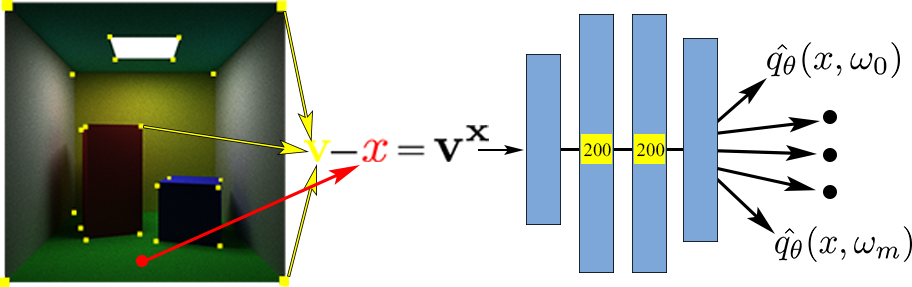
\includegraphics[width=0.9\textwidth]{images/fwd_pass_process.png}   
\caption{An illustration of the process for a forward pass on the ANN used for the Neural-Q path tracer. Starting with the scene on the left, all vertices in the scene (yellow points) are converted into a coordinate system relative to the red point $x$, producing $\mathbf{v^x}$. This is passed to the input layer of the ANN which then computes a forward pass through the two hidden layers fully connected layers, each with a width of $200$ neurons. The output layers width is equal to the number of discrete incident directions $m$ used in the approximation of the incident radiance function. Each output represents the approximated incident radiance on the position $x$ for every discrete incident direction $\hat{q_\theta}(x, \omega_k)$ $\forall k = 1, ..., m$, using parameter values $\theta$.}
\label{fig:nn_radiance_estimate_illustration}
\end{figure}

As shown in the illustration in figure \ref{fig:nn_radiance_estimate_illustration}, the ANN consists of an input layer consisting of $n$ neurons, where $n$ is the the total number of vertices in the scene. The input is then all vertices in the scene converted into a coordinate system around the intersection position $x$, $\mathbf{v^x}$. Then there are 2 hidden fully connected layers, where each hidden layer is followed by a rectifier of non-linearity activation function (ReLU) \cite{nair2010rectified}, ensuring the network can learn a non-linear function. The output layer consists of $m$ neurons to output the approximated incident radiance from every incident direction represented by discretized hemisphere around the intersection point $x$. The choice to use only two fully connected hidden layers was made to reduce time spent on computing forward passes and training the network during the rendering of an image. Whilst still having two hidden layers allows the ANN to represent an arbitrary decision boundary for approximating 5-dimensional incident radiance function $L_i(x, \omega)$, where $x \in \mathbb{R}^3$  and $\omega \in \mathbb{R}^2$. However, scenes with more complex geometry than those experimented on in chapter \ref{chap:critical_evaluation} may require more hidden layers and/or neurons in hidden layers to accurately approximate $L_i(x, \omega)$ \cite{ren2013global}.

Training the ANN is where the main difference arises compared to the supervised learning case. Recall from section \ref{sec:bootstrapping}, in the reinforcement learning case there is no large training data set available for learning the optimal value function directly. Hence, bootstrapping is used in TD-learning methods in order to learn online by continually updating the estimate of the optimal value function as data is received. This is otherwise known as learning from experience \cite{sutton2011reinforcement}. The loss function in equation \ref{eq:neural_q_loss} does exactly that, where the loss is described in terms of some immediate reward which is the emitted radiance $L_e$ term, and partially on the current estimate of incident radiance from direction $\omega$:

$$\text{TD Error: } \triangle \hat{q_\theta}(x, \omega) = \left( L_e(y, -\omega) + \left[ \max_{\omega_i} \left(\hat{q_\theta}(y, \omega_i) f_s(\omega_i, y, \omega) (\omega_i \cdot \mathbf{n}) \right) \right] \right) - \hat{q_\theta}(x, \omega)$$

So to compute this loss, an initial forward pass on the network must be made to determine the value of $\hat{q_\theta}(x, \omega)$, then a second pass must be made to calculate $max_{\omega_i} \hat{q_\theta}(y, \omega_i)$. All other terms are a result of experience and are already calculated as part of the path tracing algorithm. After the loss is calculated, backpropagation is used to compute the partial derivative of the loss with w.r.t to each parameter. Then another pass can be made through the network to update the networks weights using the partial derivatives calculated in the previous step with an optimizer. In our case we use the Adam optimizer to benefit from its use of individual learning rates for each parameter, which are adapted during learning \cite{kingma2014adam}. While there is no guarantee, in practice over many iterations of the learning procedure described, the ANNs estimate of incident radiance for a discrete set of directions $\omega_k$ for any point $x$ in the scene should move towards a local optimum \cite{deep_rl_function_approx}.

\subsection{Neural-Q Path Tracing Algorithm}

With our ANN and a method for training it to learn the the incident radiance function specified, we now present our full Neural-Q algorithm which uses the ANNs predictions for importance sampling directions to continue light paths in. Algorithm \ref{alg:neural_q_pathtracer} renders a single image using $N$ SPP to compute the colour estimate of each pixel by path tracing. Similarly to the Expected Sarsa path tracer detailed in algorithm \ref{alg:expected_sarsa_pathtracer}, the Neural-Q path tracer estimates the radiance distribution at the intersection point of a light path and samples a direction to continue the light path in proportional to this distribution. This radiance distribution is also used as the PDF for MC integration in equation \ref{eq:rendering_eq_monte_carlo} to reduce the variance in the approximation of the outgoing radiance $L_o$, leading to a reduction in image noise. Neural-Q also trains online, meaning it progressively reduces noise in the image as it simulates more light paths. Once again the $\rho_i$ term is the PDF over the hemisphere of directions $\Omega$ at intersection point $x$ to continue a light path in, evaluated for the sampled direction $\omega_i$. This can be calculated using equation \ref{eq:mc_expected_sarsa_pdf}. There are four additions made to default path tracing presented in algorithm \ref{alg:forward_path_tracing} to create the Neural-Q path tracer.

\subsubsection*{Addition 1: Minibatching}
In order to yield a smoother sampled gradient for training, a minibatching method is used where the gradient information for light paths is accumulated over a batch to train the network with. This was proven to be succesful for a range of physical control tasks in\cite{lillicrap2015continuous}. While algorithm \ref{alg:neural_q_pathtracer} iterates through the batches to clearly represent the steps the algorithm takes, in practice we performed all computation within the batch loops in parallel using a GPU.

\subsubsection*{Addition 2: Sample direction using decaying $\epsilon$-\textit{greedy} policy}
The Neural-Q path tracer follows a decaying $\epsilon$-greedy policy (see section \ref{sec:exploration_vs_exploitation}) to either exploit by sampling one of the discrete directions  proportional to the estimated radiance distribution at the intersection position. Or explore, by randomly sampling one of the discrete directions at the intersection point. This choice is made depending on the value of $\epsilon$. Where $\epsilon \in [0,1]$, a random number $r \in [0,1]$ is sampled. If $r > \epsilon$ then the so called \textit{greedy strategy} is chosen. This is where a direction is sampled proportional to the radiance distribution formed by normalizing the $m$ discrete Q-values produced by a forward pass on the network using $\mathbf{v^x}$ as input. Where each Q-value represents a discrete direction in the discretized hemisphere surrounding the intersection point $x$ of the light path. Similarly to our implementation of the  Expected Sarsa method, the hemisphere is once again discretized using the adaptive quadrature method in \cite{shirley1994notes}. in In the case of exploitation, a random direction $\omega_k$ is sampled from the discrete set directions $\omega_k$ for $i = 1,...,m$ for the adaptive quadrature at the light paths intersection point. 

\subsubsection*{Addition 3: Training the ANN}
This modification trains the ANN to improve its approximation of the incident radiance at any point $x$ in the scene, for the set of discrete angles $\omega_k$ in the adaptive quadrature centred at $x$ oriented at the surface normal at $x$. To do so, the algorithm computes the loss function in \ref{eq:neural_q_loss}, by running a forward pass on the ANN to get the approximated incident radiance in the discrete directions $\omega_k$ $\forall k=1,...,m$ for both the position $x$, as well as the next intersected position $y$. The loss is then used to train the network using the process described in section \ref{sec:ann_architecture}. The policy followed for selecting a direction to continue a light path in is different to that of selecting a direction Q-value for training with in $\hat{q_theta}(y, \omega)$ for bootstrapping. This is instead chosen according to the direction with the highest incident radiance from $y$ by following equation \ref{eq:neural_q_loss}. For this reason, the Neural-Q path tracer uses off-policy learning.

Whilst a replay buffer was not used in the Neural-Q path tracer, what it hopes to achieve is partially covered by the Neural-Q path tracing algorithm. A replay buffer was originally introduced for deep Q-learning in \cite{mnih2013playing} for training an AI agent to play a variety of Atari games by learning a good approximation of the optimal value function using deep Q-learning. The replay buffer strored transitions between state-action pairs and the corresponding reward received $e_t = (S_t, A_t, R_t, S_{t+1})$. The replay buffer is then sampled from to make up part of the minibatch to train the network with. This is known as experience replay, and is used to avoid giving the network highly correlated data to train on as a result of learning online. Training online means that taking one action in a particular state may affect the probability of selecting another action in the next state. ANNs make the assumption that the training data is independently and identically distributed (i.i.d) \cite{sutton2011reinforcement}, which was not the case for consecutive states in Atari games. Therefore, by sampling from a replay buffer, the variance in consecutive weight updates is reduced as the updates are no longer highly correlated with one another compared to using standard Q-learning \cite{sutton2011reinforcement}. 

Rather than storing transitions in a buffer to make up a minibatch for training, a batch of rays are continually traced and trained together in the Neural-Q path tracer. This avoids strong correlations between training iterations, reducing the variance in consecutive weight updates. However, it is likely there is still some correlation in the initial consecutive training iterations for light paths sampled from spatially local pixel positions in the image plane, so using some form of replay buffer like that suggested in \cite{muller2018neural} may further reduce the variance in consecutive weight updates.

\subsubsection*{Addition 4: Decaying decaying $\epsilon$-greedy}
As part of the decaying $\epsilon$-greedy policy, the value of $\epsilon$ is decreased after $1$ sampled light path is computed through every pixel in the image. Meaning, according to algorithm \ref{alg:neural_q_pathtracer}, this represents a single epoch. This is a reasonable point to decay $\epsilon$, as for an average light path length of $30$, for each sampled pixel in a $512x512$ image with a minibatch size of $1024$. Approximately $7,680$ training updates are made on the network. As discussed in section \ref{eq:exploration_vs_exploitation}, the decaying $\epsilon$-greedy policy makes sure the path tracer at first prioritises exploration of which direction contribute the most radiance. As training progresses, the path tracers policy alters more towards exploiting by sampling directions to continue light paths in based on the current estimated radiance distribution at their intersection points. This behaviour is desirable, as if we focused on exploitation to early, the path tracer may not sample seemingly unfavourable directions in the short term, which after more reflections off surfaces lead to a large amount of incident radiance to the point.

\begin{algorithm}[hbtp]
\label{alg:neural_q_pathtracer}
\SetKwProg{Fn}{Function}{ }{end}
\SetAlgoLined
 \Fn{renderImage(camera, scene, decay, $\epsilon$)}{  
   $ANN = \text{loadANN()}$\\
   \For{$i = 1$ \KwTo $N$}{
       \tcc{Addition (1)}
       \For{$b = 1$ \KwTo $\text{Batches}$}{
           \For{$k = 1$ \KwTo $\text{BatchSize}$}{
               $p \leftarrow \text{getPixel(b,k)}$\\
               $ray \leftarrow \text{initializeRay}(p, camera)$\\
               \For{$j=1$ \KwTo $\infty$}{
                   $(y, \mathbf{n}, L_e) \leftarrow \text{closestIntersection}(ray, scene)$\\
                   \If{$j > 1$}{
                       \tcc{Addition (2)}
                       $(\omega_i, \rho_i, f_s) \leftarrow \text{sampleRayDirEpsilonGreedy}(\epsilon, y)$\\
                       \tcc{Addition (3)}
                       $\hat{q_\theta}x \leftarrow ANN.getQValue(ray.x, ray.\omega, scene)$\\
                       $\hat{q_\theta}y \leftarrow ANN.getMaxQValue(y, scene)$\\
                       $\triangle \hat{q}_\theta x \leftarrow L_e +  \left(\hat{q_\theta}y  \cdot f_s \cdot (\omega_i \cdot \mathbf{n}) \right) - \hat{q_\theta}x$\\
                       $ANN.\text{train}(\triangle \hat{q}_\theta x)$
                   }
                   \If{$\text{noIntersection}(y) \ \Or \ \text{areaLightIntersection}(y)$}{
                       $ray.throughput \leftarrow ray.throughput \cdot L_e$\\
                       $\text{updatePixelColourEstimate}(p, ray.throughput)$\\
                       $\Break$
                   }
                  $ray.throughput \leftarrow ray.throughtput \cdot f_s \cdot (\omega_i \cdot \mathbf{n}) / \rho_i$\\
                  $ray \leftarrow (y, \omega_i)$
               }
           }
       }
       \tcc{Addition (4)}
       $\epsilon \leftarrow \epsilon - decay$
   }
 }
 \caption{Neural-Q forward path tracer. Given a camera position, scene geometry, epsilon and epsilon decay, this algorithm will render a single image. Where $N$ is the pre-specified number of sampled light paths per pixel. The algorithm trains the ANN online to progressively reduce noise in consecutive rendered images, by improving its approximation of the incident radiance function for the scene.}
\end{algorithm}


\begin{comment}
% Advantages
% Less memory
% Same architecture can be applied to scene rather then applying complex data structures to the scene

Deep Learning for denoising light transport simulation rendering methods:
\begin{itemize}
\item \cite{zheng2018learning} - Uses a DNN to pre-train on a scene to figure out which pixels require more samples rather then just uniformly sampling the same amount of light rays for every pixel.

\item \cite{muller2018neural} - Uses a DNN for both online learning in light path construction and also introduces i for Primary Sample Space importance sampling. Performs well, not usable currently due to bottleneck of inference

"At any given point during rendering, a sample is generated by drawing a random pair u ∈ [0, 1] passing it through the inverted coupling layers in reverse order, and transforming to the range of cylindrical coordinates to obtain ω." - This means it simply gives a direction rather then return the value of directions around it, does this mean there is no stochasticity when sampling a new direction? Everytime we intersect with a world coordinate we will sample a ray in the same direction if no training occurs? Dont make this claim just allude to importance sampling over directions is better

\item \cite{keller2019integral} - Introduces a range of methods for NN, most related to mine is using NN to output Q-value of the light source. Neural network determines which light source to compute direct illumination from for a given normal, intersection point and incoming direction to the intersection point. They also use it to determine visibility, which light sources contribute the most to a point, as well as a direct approximation of radiance
\end{itemize}


{\bf A topic-specific chapter, of roughly $15$ pages} 
\vspace{1cm} 

\noindent
This chapter is intended to describe what you did: the goal is to explain
the main activity or activities, of any type, which constituted your work 
during the project.  The content is highly topic-specific, but for many 
projects it will make sense to split the chapter into two sections: one 
will discuss the design of something (e.g., some hardware or software, or 
an algorithm, or experiment), including any rationale or decisions made, 
and the other will discuss how this design was realised via some form of 
implementation.  

This is, of course, far from ideal for {\em many} project topics.  Some
situations which clearly require a different approach include:

\begin{itemize}
\item In a project where asymptotic analysis of some algorithm is the goal,
      there is no real ``design and implementation'' in a traditional sense
      even though the activity of analysis is clearly within the remit of
      this chapter.
\item In a project where analysis of some results is as major, or a more
      major goal than the implementation that produced them, it might be
      sensible to merge this chapter with the next one: the main activity 
      is such that discussion of the results cannot be viewed separately.
\end{itemize}

\noindent
Note that it is common to include evidence of ``best practice'' project 
management (e.g., use of version control, choice of programming language 
and so on).  Rather than simply a rote list, make sure any such content 
is useful and/or informative in some way: for example, if there was a 
decision to be made then explain the trade-offs and implications 
involved.

\section{Example Section}

This is an example section; 
the following content is auto-generated dummy text.
\lipsum

\subsection{Example Sub-section}

\begin{figure}[t]
\centering
foo
\caption{This is an example figure.}
\label{fig}
\end{figure}

\begin{table}[t]
\centering
\begin{tabular}{|cc|c|}
\hline
foo      & bar      & baz      \\
\hline
$0     $ & $0     $ & $0     $ \\
$1     $ & $1     $ & $1     $ \\
$\vdots$ & $\vdots$ & $\vdots$ \\
$9     $ & $9     $ & $9     $ \\
\hline
\end{tabular}
\caption{This is an example table.}
\label{tab}
\end{table}

\begin{algorithm}[t]
\For{$i=0$ {\bf upto} $n$}{
  $t_i \leftarrow 0$\;
}
\caption{This is an example algorithm.}
\label{alg}
\end{algorithm}

\begin{lstlisting}[float={t},caption={This is an example listing.},label={lst},language=C]
for( i = 0; i < n; i++ ) {
  t[ i ] = 0;
}
\end{lstlisting}

This is an example sub-section;
the following content is auto-generated dummy text.
Notice the examples in Figure~\ref{fig}, Table~\ref{tab}, Algorithm~\ref{alg}
and Listing~\ref{lst}.
\lipsum

\subsubsection{Example Sub-sub-section}

This is an example sub-sub-section;
the following content is auto-generated dummy text.
\lipsum

\paragraph{Example paragraph.}

This is an example paragraph; note the trailing full-stop in the title,
which is intended to ensure it does not run into the text.


\subsection{Plan}

% I imagine this section to be like a mini paper starting at new method

\textbf{Breakdown}
\begin{enumerate}

\item State learning rule for deep Q-learning and the difference from deep Q-learning to q-learning. Maybe some of the difficulties associated with deep q-learning versus q-learning, and some of the general advantages. 

\item Derive the learning rule for deep q-learning network which I used, once again justifying terms throughout the derivation.

\item Explain concept of eta-greedy policy used. Explain exploration vs exploitation but we will talk about this more later

\item Describe how the current method is used for diffuse surfaces. Introduce the pseudo code for the new algorithm. Give a description of each stage and what it does. Relating back to properties such as bias rendering and pointing out assumption made by the path tracer.

\item Present and explain the network architecture. Explain in depth about how the state was modelled as a point relative to all vertices to give the network information about the position of the vertex relative to the rest of the world compared to passing in a single position. Relate this to Atari games, we get an image showing where we are relative to the world rather than just a single position in the world.

\item Present some results side by side against a default path tracer and Nvidia's reinforcement learning approach. Pointing out aspects of the image and reasoning for certain parts.

\end{enumerate}
\end{comment}

\end{document}